\documentclass[accentcolor=tud6b,colorbacktitle,inverttitle,landscape,german,presentation,t]{tudbeamer}
\usepackage[T1]{fontenc} 
\usepackage[utf8]{inputenc} 
\usepackage[ngerman]{babel}
\usepackage{listings}
\usepackage{pdfpages}
\usepackage{mathtools}
\usepackage[]{algorithm2e}
\usepackage{rotating}
\usepackage{multirow}
\usepackage{pdfpages}
\usepackage{epstopdf}

\begin{document}

\title[Klassifikation der Schwierigkeitsgrade von Sudokus mit Methoden des maschinellen Lernens]{Päsentation Bachelorarbeit}
\subtitle{Michael Bräunlein\\mbraeunlein@gmail.com}

\author[M. Bräunlein]{Michael Bräunlein}
\institute[Knowledge Engineering TUD]{Knowledge Engineering, TU Darmstadt}

\logo{
\includegraphics{TUDbeamer-logo}}

\date{17 April 2014}

\begin{titleframe}
\centering \LARGE Klassifikation der Schwierigkeitsgrade von Sudokus mit Methoden des maschinellen Lernens
\end{titleframe}

\section{Einleitung}
	\begin{frame}
	\frametitle{Einleitung}
	\begin{itemize}
	\item Sudokus finden sich überall
	\item Unterschiedliche Bewertungsskalen
	\item Unterschiedliche Einteilungsverfahren
	\item Bisher kein Verfahren zur Einteilung mit maschinellem Lernen
	\item Sudokus sind zur Bearbeitung mit Computern prädestiniert
	\end{itemize}
	\end{frame}

\section{Grundlagen}
	\subsection{Regeln}
		\begin{frame}
		\frametitle{Die Regeln}
		\begin{itemize}
		\item Sudoku hat nur eine Regel
		\item In jeder Zeile, jeder Spalte und jedem Block muss jede Ziffer von 1 bis 9 genau einmal vorkommen
		\item Jedes Sudoku hat eine eindeutige Lösung
		\item Das Sudoku gilt dann als gelöst, wenn alle Felder ausgefüllt sind
		\end{itemize}
		\end{frame}

	\subsection{Lösungsmethoden}
		\begin{frame}
		\frametitle{Lösungmethoden}
		\begin{itemize}
		\item Lösungsmethoden sagen viel über den Schwierigkeitsgrad aus
		\item Jeder Spieler benutzt Lösungsmethoden
		\item Kandidatenlisten erleichtern das Finden von Zahlenkonstellationen, die Voraussetzung für bestimmte Lösungsmethoden sind
		\item Es gibt viele verschiedene Lösungsmethoden, grob werden zwei Kategorien unterschieden
		\end{itemize}
		\begin{figure}[Hh]
    		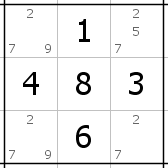
\includegraphics[width=\textwidth-270pt,height=\textheight,keepaspectratio]{./img/kandidatenlisten.png}
		\end{figure}
		\end{frame}

		\subsubsection{Hidden Single}
			\begin{frame}
			\frametitle{Hidden Single}
			\begin{figure}[Hh]
    			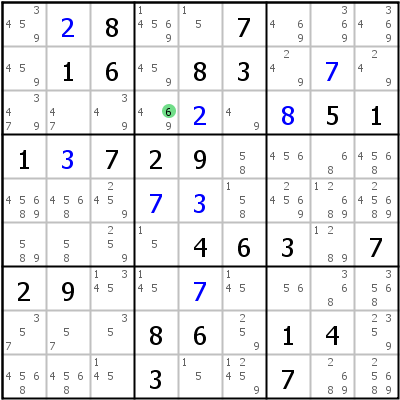
\includegraphics[width=\textwidth,height=\textheight-10pt,keepaspectratio]{./img/hidden_single.png}
			\end{figure}
			\end{frame}

		\subsubsection{Pointing Pair / Triple}
			\begin{frame}
			\frametitle{Pointing Pair / Triple}
			\begin{figure}[Hh]
    			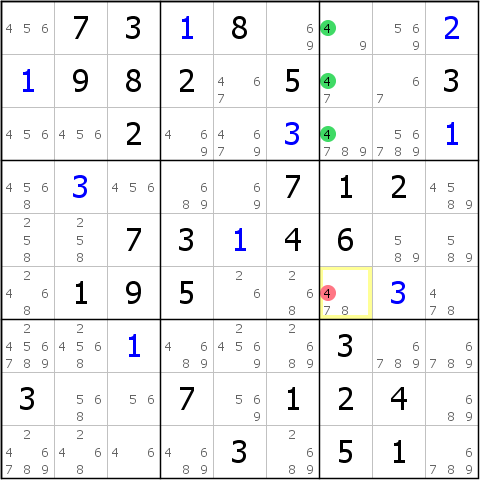
\includegraphics[width=\textwidth,height=\textheight-10pt,keepaspectratio]{./img/pointing_triple.png}
			\end{figure}
			\end{frame}

		\subsubsection{Two-String-Kite}
			\begin{frame}
			\frametitle{Two-String-Kite}
			\begin{figure}[Hh]
    			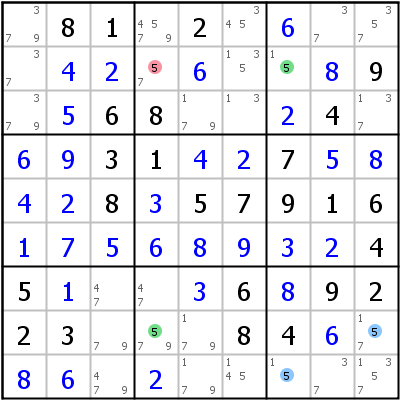
\includegraphics[width=\textwidth,height=\textheight-10pt,keepaspectratio]{./img/2stringkite.png}
			\end{figure}
			\end{frame}

		\subsubsection{XY-Wing}
			\begin{frame}
			\frametitle{XY-Wing}
			\begin{figure}[Hh]
    			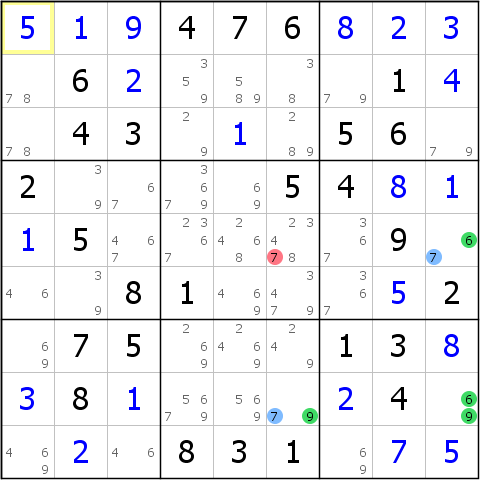
\includegraphics[width=\textwidth,height=\textheight-10pt,keepaspectratio]{./img/XY_Wing.png}
			\end{figure}
			\end{frame}

\section{Klassifikation}
	\subsection{Was sind Featurevectoren}
		\begin{frame}
		\frametitle{Was sind Featurevectoren}
		\begin{itemize}
		\item Merkmalsvektor
		\item n-dimensionaler Vektor
		\item Repräsentation eines Objekts
		\item Ein Eintrag steht für eine Eigenschaft des beschriebenen Sudokus
		\item Featurevektoren sind die Eingabe des Klassifikationsalgorithmus
		\end{itemize}
		\end{frame}

	\subsection{Wie werden Featurevectoren erzeugt}
		\begin{frame}
		\frametitle{Wie werden Featurevectoren erzeugt}
		\begin{itemize}
		\item Am Anfang bekannte Zahlen
		\item Einträge der Kandidatenlisten
		\item Hinzugefügte Zahlen
		\item Entfernte Zahlen
		\item Unterschiedliche Lösungswege für Sudokus möglich
		\item Einfachster Lösungsweg gesucht
		\item Ungelöste Felder
		\item Insgesammt 261 Features
		\end{itemize}
		\end{frame}

%%%%%%%%%%%%%%%%%%% Eine Folie mit Effekt %%%%%%%%%%%%%%%%%%%
	\subsection{Entkopplung von konkreten Zahlen}
		\begin{frame}
		\frametitle{Entkopplung von konkreten Zahlen}
		\begin{itemize}
		\item Fast gleiche Sudokus mit vertauschten Zahlen
		\item Gleicher Schwierigkeitsgrad
		\item Unterschiedliche Featurevectoren bei gleichem Lösungsweg
		\end{itemize}
		\end{frame}
	\subsection{Entkopplung von konkreten Zahlen}
		\begin{frame}
		\frametitle{Entkopplung von konkreten Zahlen}
		\begin{itemize}
		\item Fast gleiche Sudokus mit vertauschten Zahlen
		\item Gleicher Schwierigkeitsgrad
		\item Unterschiedliche Featurevectoren bei gleichem Lösungsweg
		\item Lösung?
		\end{itemize}
		\end{frame}
	\subsection{Entkopplung von konkreten Zahlen}
		\begin{frame}
		\frametitle{Entkopplung von konkreten Zahlen}
		\begin{itemize}
		\item Fast gleiche Sudokus mit vertauschten Zahlen
		\item Gleicher Schwierigkeitsgrad
		\item Unterschiedliche Featurevectoren bei gleichem Lösungsweg
		\item Sortierung der Features nach Häufigkeit
		\item Kein relevanter Informationsverlust
		\item Gleicher Featurevector auch bei vertauschten Ziffern
		\end{itemize}
		\end{frame}
%%%%%%%%%%%%%%%%%%%%%%%%%%%%%%%%%%%%%%%%%%%%%%

	\subsection{Entkopplung von konkreten Zahlen (Beispiel)}
		\begin{frame}
		\frametitle{Entkopplung von konkreten Zahlen (Beispiel)}
		\begin{itemize}
		\item Beispiel des Featurevectors einer Methode\\$\mathbf{(1, 0, 4, 15, 3, 0, 9, 2, 0)^{T}}$
		\item Vertauchte Ziffern 7 und 8\\$\mathbf{(1, 0, 4, 15, 3, 0, 2, 9, 0)^{T}}$
		\item Nach der Sortierung nach der Häufigkeit\\$\mathbf{(15, 9, 4, 3, 2, 1, 0, 0, 0)^{T}}$
		\end{itemize}
		\end{frame}

\section{Ergebnisse}
	\subsection{Software}
		\begin{frame}
		\frametitle{Software}
		\begin{itemize}
		\item Fremdsoftware für Klassifizierer und Lösungsmethoden
		\item Für den Klassifizierer: Weka\footnote{\url{http://www.cs.waikato.ac.nz/ml/weka/}}, J48 Klassifizierer
		\item Für die Lösungsmethoden: Hodoku\footnote{\url{http://hodoku.sourceforge.net/de/index.php}}
		\item Beide Projekte stehen unter der GPLv3 Lizenz
		\item Eigene Software in Java
		\item Extrahierung der Featurevectoren und Verbindung der Projekte
		\end{itemize}
		\end{frame}

	\subsection{J48 Klassifizierer}
		\begin{frame}
		\frametitle{J48 Klassifizierer}
		\begin{itemize}
		\item Genauer Algorithmus, der auch Einblicke in die Klassifikationsgrundlage liefert
		\item Erstellt mit den Trainingsdaten einen Entscheidungsbaum
		\end{itemize}
		\begin{figure}[Hh]
    		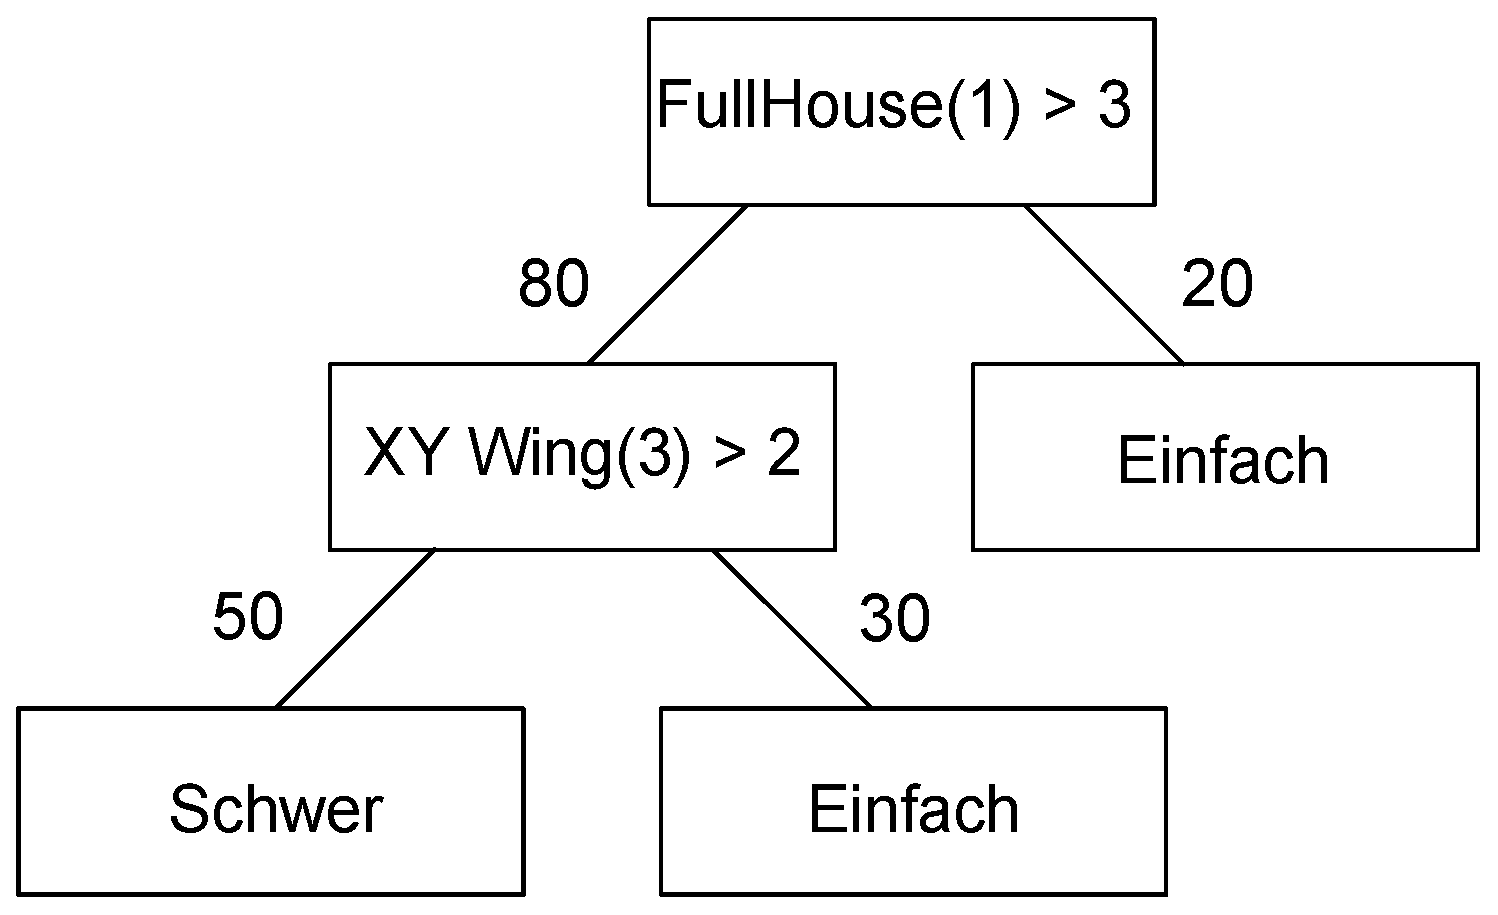
\includegraphics[width=\textwidth - 150pt,height=\textheight-10pt,keepaspectratio]{./img/entscheidungsbaum.eps}
		\end{figure}
		\end{frame}

	\subsection{J48 Klassifizierer}
		\begin{frame}
		\frametitle{J48 Klassifizierer}
		\begin{itemize}
		\item J48 erhält 2 Parameter C und M für postpruning
		\item Je kleiner C, desto eher wird der Baum abgeschnitten
		\item Je größer M, desto mehr Instanzen müssen sich mindestens in einem Blatt befinden
		\item Optimierung der Parameter für das verwendete Testset
		\item 1000 Auswertungen von Parameterkombinationen
		\item Optimum bei C: 0.1 und M: 30
		\end{itemize}
		\end{frame}

	\subsection{Optimierung der Parameter}
		\begin{frame}
		\frametitle{Optimierung der Parameter}
		\begin{figure}[Hh]
    		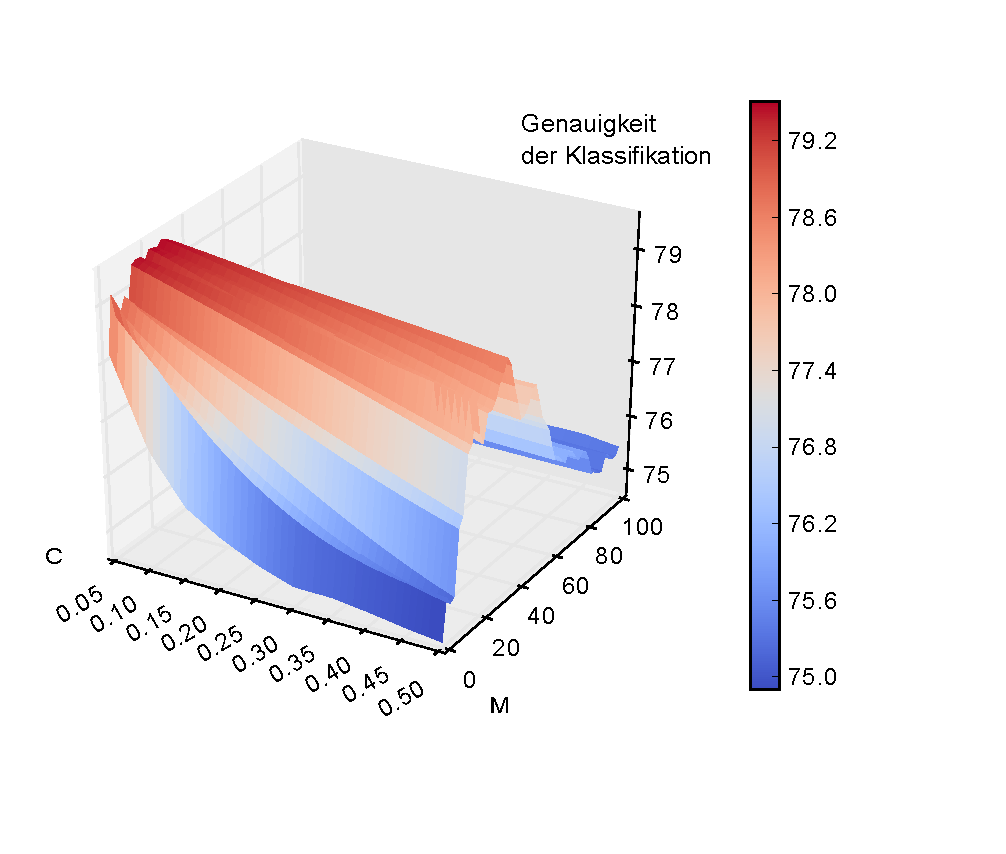
\includegraphics[width=\textwidth,height=\textheight,keepaspectratio]{./img/parameter.eps}
		\end{figure}
		\end{frame}

	\subsection{Evaluierung des Featurevectors}
		\begin{frame}
		\frametitle{Evaluierung des Featurevectors}
		\begin{figure}[Hh]
		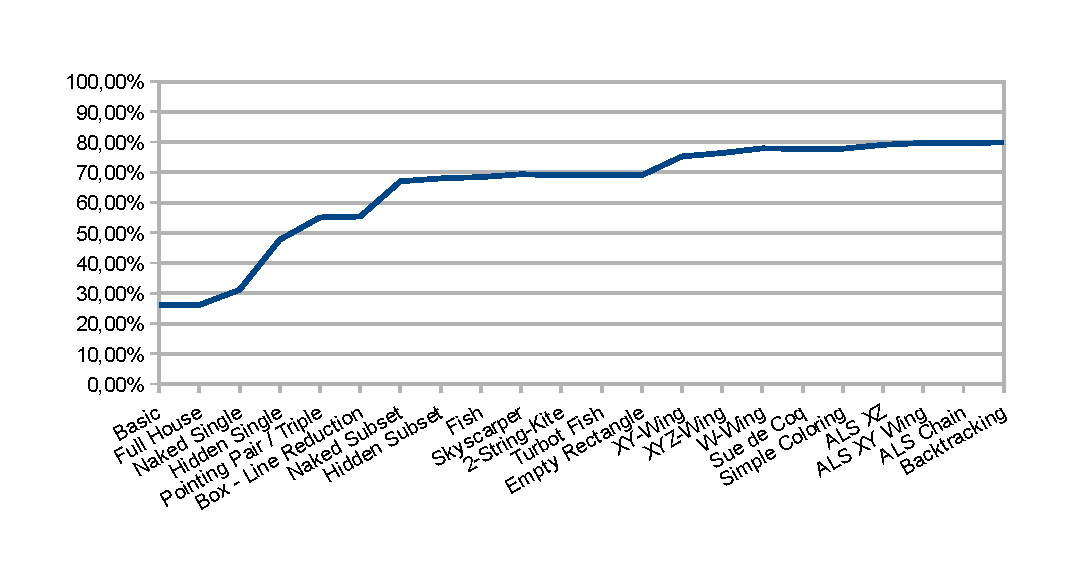
\includegraphics[width=\textwidth,height=\textheight,keepaspectratio]{./img/accuracy.eps}
		\end{figure}
		\end{frame}

	\subsection{Evaluierung des Featurevectors}
		\begin{frame}
		\frametitle{Evaluierung des Featurevectors}
		\begin{figure}[Hh]
		\centering
		\begin{tabular}{ l | l |  c  c  c  c  c | l}
		\multicolumn{7}{c}{\textbf{Zugeordnete Klasse}}\\
		\cline{2-7}
		\multirow{6}{*}{\begin{turn}{90}\textbf{Klasse}\end{turn}}
		 &  & a & b & c & d & e\\
		\cline{2-7}
		& a & 1000 & 0 & 0 & 0 & 0 & a = Easy \\
		& b & 0 & 568 & 115 & 93 & 224 & b = Middle \\
		& c & 0 & 288 & 333 & 221 & 158 & c = Hard \\
		& d & 0 & 309 & 257 & 225 & 209 & d = Unfair \\
		& e & 0 & 415 & 149 & 177 & 259 & e = Extreme \\
		\cline{2-7}
		\end{tabular}
		\caption{Konfustionsmatrix mit einschließlich \textit{Hidden Single} Methode}
		\end{figure}
		\end{frame}

	\subsection{Evaluierung des Featurevectors}
		\begin{frame}
		\frametitle{Evaluierung des Featurevectors}
		\begin{figure}[Hh]
		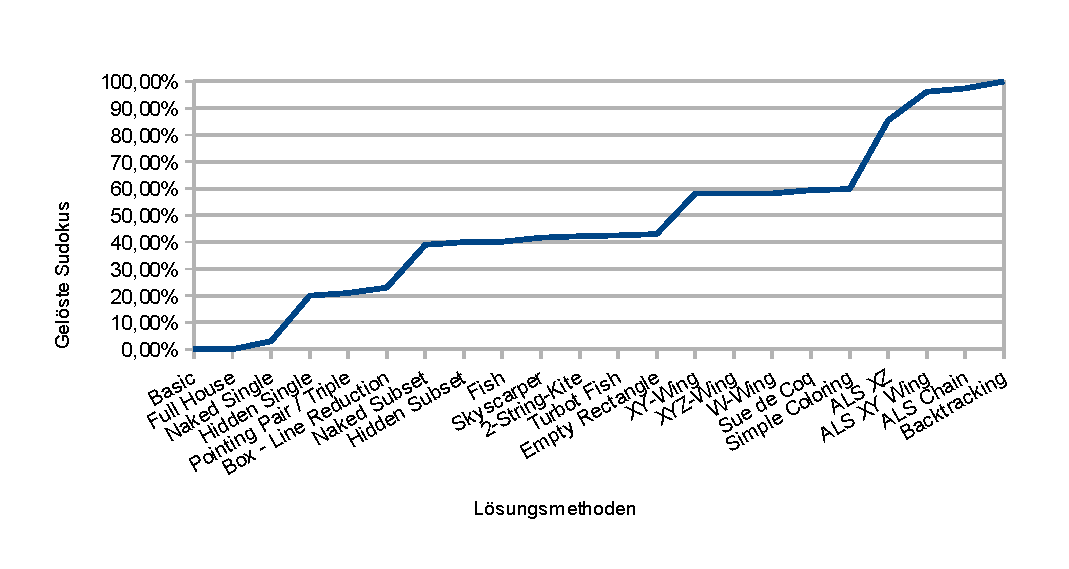
\includegraphics[width=\textwidth,height=\textheight,keepaspectratio]{./img/solvedcount.eps}
		\end{figure}
		\end{frame}

	\subsection{Evaluierung des Featurevectors}
		\begin{frame}
		\frametitle{Evaluierung des Featurevectors}
		\begin{figure}[Hh]
		\centering
		\begin{tabular}{ l | l |  c  c  c  c  c | l}
		\multicolumn{7}{c}{\textbf{Zugeordnete Klasse}}\\
		\cline{2-7}
		\multirow{6}{*}{\begin{turn}{90}\textbf{Klasse}\end{turn}}
		 &  & a & b & c & d & e\\
		\cline{2-7}
		& a & 1000 & 0 & 0 & 0 & 0 & a = Easy \\
		& b & 0 & 999 & 1 & 0 & 0 & b = Middle \\
		& c & 1 & 35 & 785 & 145 & 34 & c = Hard \\
		& d & 0 & 10 & 129 & 636 & 225 & d = Unfair \\
		& e & 0 & 0 & 14 & 367 & 619 & e = Extreme \\
		\cline{2-7}
		\end{tabular}
		\caption{Konfustionsmatrix mit allen vorgestellten Lösungsmethoden}
		\end{figure}
		\end{frame}

	\subsection{Mapping}
		\begin{frame}
		\frametitle{Mapping}
		\begin{itemize}
		\item Vergleich verschiedener Bewertungsskalen
		\item Trainieren einen Klassifizierers mit einem Trainingsset
		\item Klassifizieren eines zweiten Sets mit dem gelernten Entscheidungsbaum
		\item Zur Verifikation Datensets vertauschen
		\item Darstellung der Ergebnisse als Matrix
		\end{itemize}
		\end{frame}

	\subsection{Mapping Matrix}
		\begin{frame}
		\frametitle{Mapping Matrix}
		\begin{figure}[Hh]
		\centering
		\begin{tabular}{ l | l |  c  c  c  c  c |}
		\multicolumn{7}{c}{\textbf{Zugeordnete Klasse}}\\
		\cline{2-7}
		\multirow{6}{*}{\begin{turn}{90}\textbf{Ursprüngliche Klasse}\end{turn}}
 		&  & Easy & Middle & Hard & Unfair & Extreme\\
		\cline{2-7}
		& Sehr Einfach & 32 & 0 & 0 & 0 & 0\\
		& Einfach & 32 & 0 & 0 & 0 & 0\\
		& Standard & 32 & 0 & 0 & 0 & 0\\
		& Moderat & 0 & 32 & 0 & 0 & 0\\
		& Anspruchsvoll & 0 & 1 & 30 & 1 & 0\\
		& Sehr Anspruchsvoll & 0 & 1 & 28 & 2 & 1\\
		& Teuflisch & 0 & 0 & 7 & 8 & 17\\
		\cline{2-7}
		\end{tabular}
		\end{figure}
		\end{frame}

	\subsection{Relative Güte der Features}
		\begin{frame}
		\frametitle{Relative Güte der Features}
		\begin{itemize}
		\item Manche Features bieten mehr Informationen als andere
		\item Wichtigere Features stehen weiter oben im Entscheidungsbaum
		\item Unwichtige Features können auch gar nicht im Baum vorkommen
		\item J48 benutzt postpruning
		\item Evaluierung der wichtigen Features kann den Featurevector schmaler machen und dadurch die Laufzeit beim Erstellen des Entscheidungsbaums verbessern
		\item Finden der wichtigen Features mit CFS
		\item18 von 261 Features ausgewählt, Genauigkeitsverlust von 1\%
		\end{itemize}
		\end{frame}

	\subsection{Relative Güte der Features (ALS XZ)}
		\begin{frame}
		\frametitle{Relative Güte der Features (ALS XZ)}
		\begin{figure}[Hh]
		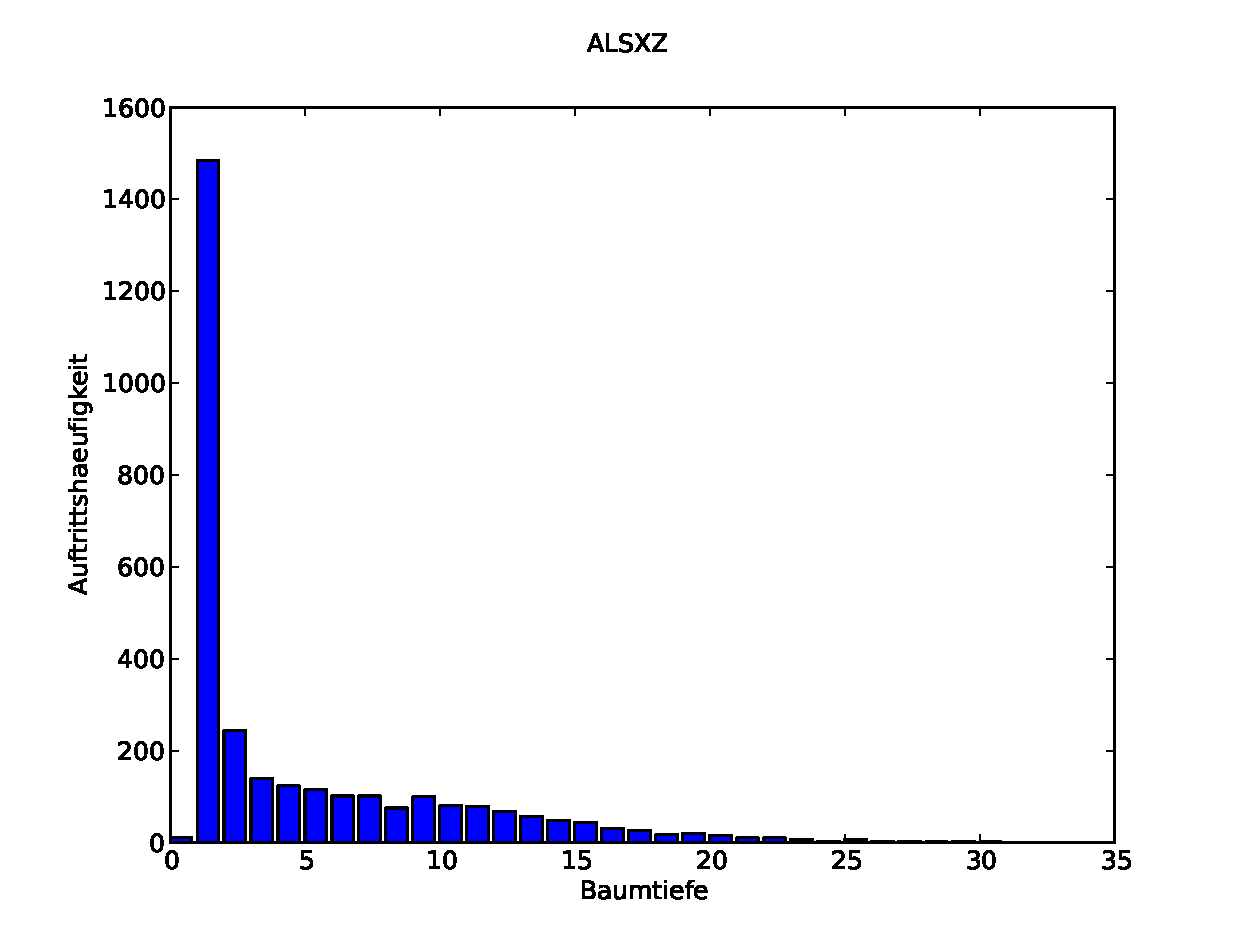
\includegraphics[width=\textwidth,height=\textheight,keepaspectratio]{./img/ALSXZ_hist.eps}
		\end{figure}
		\end{frame}

	\subsection{Relative Güte der Features (Sue de Coq)}
		\begin{frame}
		\frametitle{Relative Güte der Features (Sue de Coq)}
		\begin{figure}[Hh]
		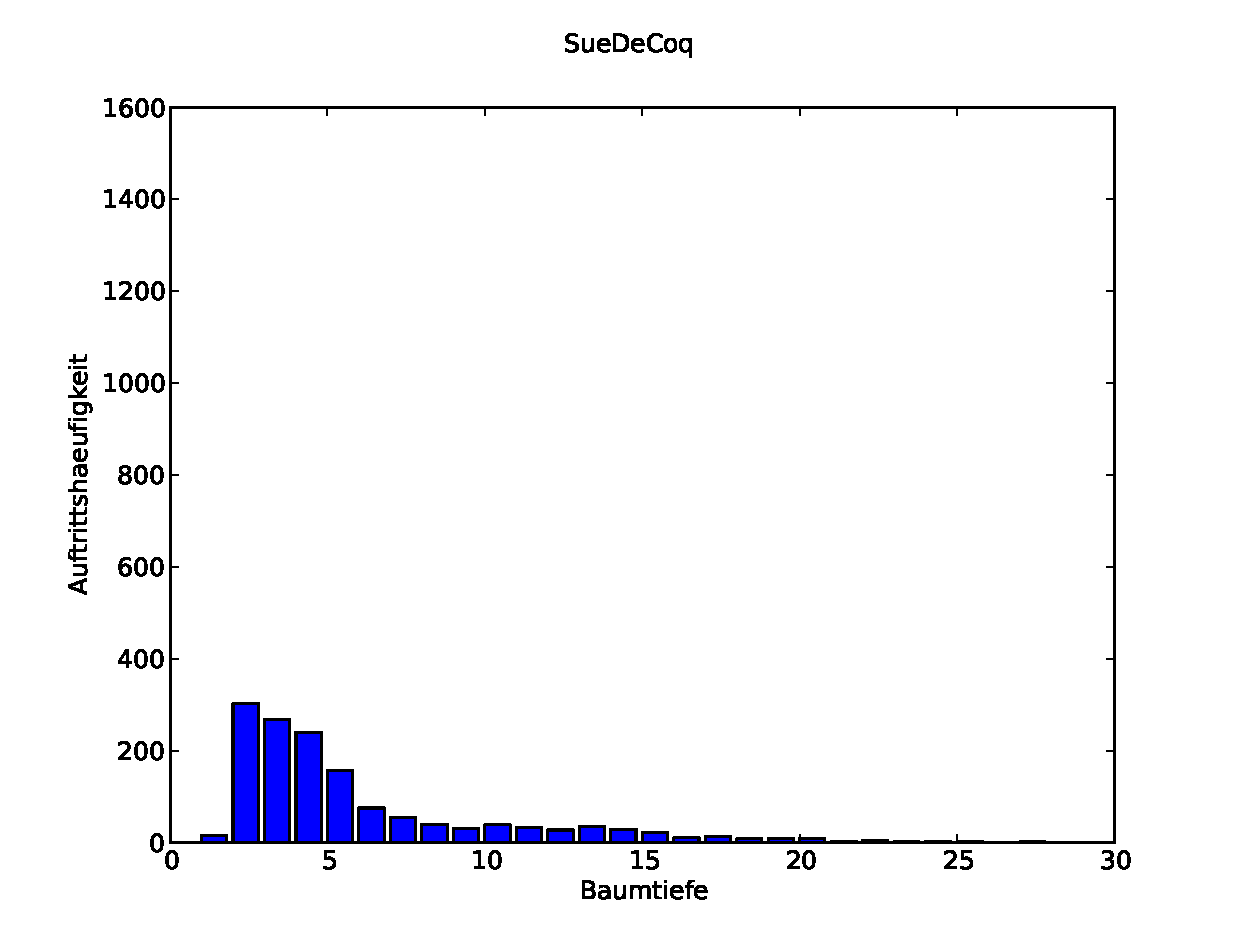
\includegraphics[width=\textwidth,height=\textheight,keepaspectratio]{./img/SueDeCoq_hist.eps}
		\end{figure}
		\end{frame}

	\subsection{Relative Güte der Features (Hidden Quadruples)}
		\begin{frame}
		\frametitle{Relative Güte der Features (Hidden Quadruples)}
		\begin{figure}[Hh]
		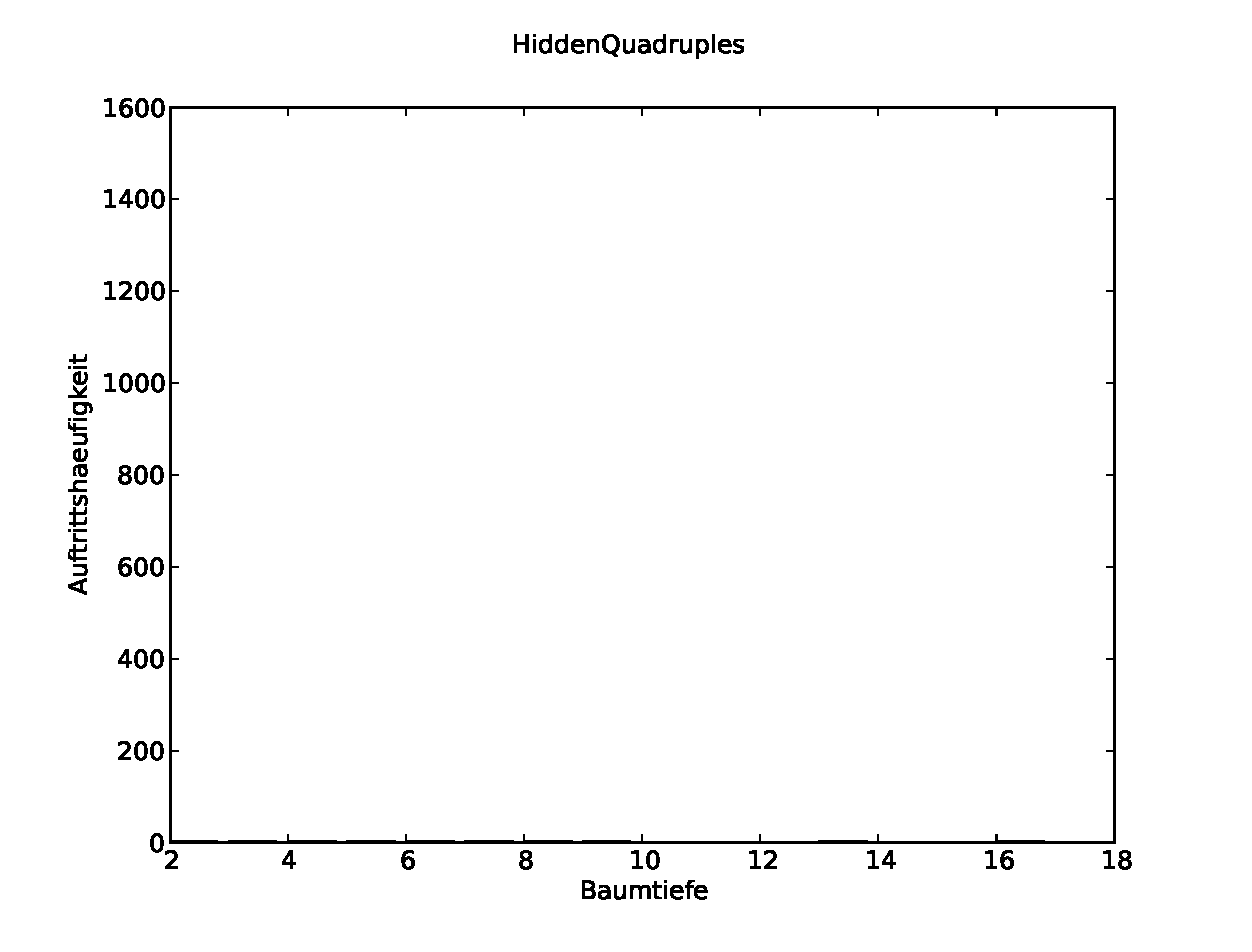
\includegraphics[width=\textwidth,height=\textheight,keepaspectratio]{./img/HiddenQuadruples_hist.eps}
		\end{figure}
		\end{frame}

\section{Zusammenfassung und Ausblick}
	\subsection{Zusammenfassung}
		\begin{frame}
		\frametitle{Zusammenfassung}
		\begin{itemize}
		\item Erstellen eines Featurevectors
		\item Entkopplung von konkreten Zahlen
		\item Klassifikation mit J48
		\item Genauigkeit von ca. 80\%
		\item Optimierung der Parameter
		\item Identifikation von Features die mehr Informationsgewinn liefern
		\item Mapping verschiedener Bewertungsskalen
		\end{itemize}
		\end{frame}

	\subsection{Ausblick}
		\begin{frame}
		\frametitle{Ausblick}
		\begin{itemize}
		\item Entwicklung neuer Features z.B. Zeit, die ein menschlicher Spieler zum Lösen benötigt
		\item Verwendung von mehr Lösungsmethoden
		\item Evaluierung anderer Klassifikationsalgorithmen
		\item Qualitätsevaluation des Mappingverfahrens
		\end{itemize}
		\end{frame}

\section{Literaturverzeichnis} 
	\begin{thebibliography}{10} 
	\bibitem{hall1998}Hall, M., A.: {\glqq Correlation-based Feature Subset Selection for Machine Learning \grqq}. University of Waikato, 1998. 
	\bibitem{witten2011}Witten, I., H.; Frank, E.; Hall, M., A.: {\glqq Data Mining: Practical Machine Learning Tools and Techniques - Practical Machine Learning Tools and Techniques \grqq}. 3. Auflage, Elsevier Amsterdam, 2011. 
	\end{thebibliography}

\section{Ende}
	\subsection{Ende}
		\begin{frame}
		\frametitle{Ende...}
		\begin{figure}[Hh]
		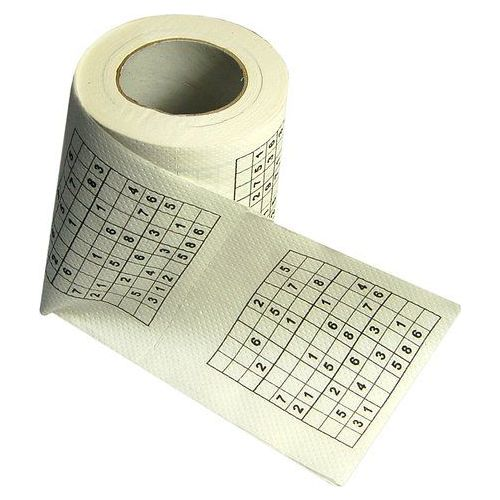
\includegraphics[width=\textwidth,height=\textheight,keepaspectratio]{./img/title.jpg}
		\end{figure}
		\end{frame}



\end{document}

